\section{Methodology and Test Framework}
\label{sec:methodology}

A dual-rate simulation framework separates continuous-time system
physics ($f_{\mathrm{s,phys}}=1$\,MHz) from discrete-time estimation
($f_{\mathrm{s,DSP}}=10$\,kHz). This yields negligible numerical error in
ground-truth frequency trajectories while reproducing the sampling
constraints of commercial protection relays.

% ---------------------------------------------------------
\subsection{Evaluated Estimators}
% ---------------------------------------------------------

Twelve estimators from five algorithmic families are evaluated
(Table~\ref{tab:unified_2024_big}). \textbf{Loop-based:} SRF-PLL and
SOGI-FLL with PI gains, IIR bandpass pre-filter, and FastRMS adaptive
amplitude normalizer (not a standard textbook SOGI-FLL~\cite{Golestan2015}).
A unit inconsistency in the SOGI-FLL adaptation law (rad/s vs.\ Hz,
factor $120\pi\,\text{rad/s}$) was identified and corrected prior to
evaluation. The narrow effective passband created by the bandpass
pre-filter and adaptive normalizer suppresses apparent frequency
deviation under a phase jump but cannot track sustained linear RoCoF,
explaining the divergent ranking across Scenarios~B and~D.
\textbf{Window-based:} IpDFT with a Hann window and three-point
magnitude-parabolic interpolation~\cite{Quinn1994}
(the complex Jacobsen estimator is unsuitable here because
Hann-window sidelobes are negative-real, which inverts the interpolation
direction); TFT with a 2nd-order Taylor-series expansion of
the fundamental component, Hann-weighted, which improves RoCoF tracking
relative to a static DFT at the cost of higher noise
sensitivity~\cite{PlatasGarza2011}. \textbf{Adaptive recursive:} RLS and
VFF-RLS with a 2nd-order AR(2) bandpass pre-whitening filter.
\textbf{Data-driven:} Koopman (RK-DPMU) and PI-GRU.
\textbf{Model-based:} EKF, UKF, and RA-EKF. The column ``RoCoF Out.''
indicates whether RoCoF is available as an explicit output~(S) or
derived by implicit differentiation~(D). The UKF includes a 10-sample
output moving average not present in the classic EKF.

% ---------------------------------------------------------
\subsubsection{Implemented RA-EKF Estimator}
% ---------------------------------------------------------

RoCoF state augmentation in the EKF has been studied
previously~\cite{Ferrero2020EKF,Chamorro2021}. The RA-EKF uses a 4-state
vector $[\theta_k,\omega_k,A_k,\dot{\omega}_k]^\top$ with second-order
kinematic prediction ($\theta_k = \theta_{k-1}+\omega_{k-1}\Delta t +
\tfrac{1}{2}\dot{\omega}_{k-1}\Delta t^2$; $\omega_k = \omega_{k-1}+\dot{\omega}_{k-1}\Delta t$)
and two IBR-tailored mechanisms.
\emph{Innovation-Driven Covariance Scaling:}
$\mathbf{Q}_k = \mathrm{clip}(r_k,0.25,4)\,\mathbf{Q}_{\mathrm{base}}$,
where $r_k = |\nu_k|/\hat{\sigma}_\nu$, inflates process noise during
transients and reduces it at steady state.
\emph{Event Gating:}
when $|\nu_k|>\gamma\hat{\sigma}_\nu$ ($\gamma=2.0$), a soft
re-initialization updates $\theta_k$ only, preserving $\omega_k$ and
$\dot{\omega}_k$ to limit cycle-slip behavior at phase discontinuities.
This heuristic trades strict stochastic optimality for bounded nonlinear
stability during abrupt phase steps.

% ---------------------------------------------------------
\subsection{Test Scenarios and Noise Model}
\label{sec:scenarios}
% ---------------------------------------------------------

Five scenarios stress the estimators under representative IBR-grid
conditions (Fig.~\ref{fig:scenarios}). Tests~(A)--(C) use Additive White
Gaussian Noise (AWGN) with
$\sigma=0.001$\,pu; Scenario~(D) uses $\sigma=0.005$\,pu; and
Scenario~(E) uses $\sigma=0.003$\,pu base noise plus sparse impulsive
samples (amplitude $\leq0.05$\,pu, probability $<1\%$).
%
\begin{itemize}[leftmargin=*, nosep, topsep=1pt, itemsep=1pt]
  \item[\textbf{(A)}] \textbf{Magnitude Step:} $+10\%$ voltage step with
    zero phase angle at the disturbance onset.
  \item[\textbf{(B)}] \textbf{Frequency Ramp:} $+3.0$\,Hz/s RoCoF (IEEE 1547-2018 Category III compliant).
  \item[\textbf{(C)}] \textbf{AM Modulation:} 10\% depth at 2\,Hz.
  \item[\textbf{(D)}] \textbf{Composite Islanding:} instantaneous
    $+60^\circ$ phase jump (maximum mismatch during breaker
    reclosing~\cite{Roscoe2019}), 4\% 5th harmonic (250\,Hz), 2\% 7th
    harmonic (350\,Hz), 0.5\% 32.5\,Hz interharmonic
    (a sub-synchronous component characteristic of IBR converter switching;
    Total Harmonic Distortion THD\,$\approx$\,4.5\%, IEEE~519 compliant),
    and $\sigma=0.005$\,pu noise.
  \item[\textbf{(E)}] \textbf{IBR Multi-Event:} 5\,s sequence with
    harmonic-rich steady state (5th: 4\%, 7th: 2\%;
    THD\,$\approx$\,4.5\%, IEEE~519 compliant), a $+40^\circ$
    phase jump, a $-3.0$\,Hz/s RoCoF segment reaching a nadir of
    $57.5$\,Hz (IEEE~1547-2018 UFLS limit), a $+80^\circ$ jump with
    second-order ring-down recovery, and impulsive noise~\cite{Chamorro2021}.
\end{itemize}
%
Scenarios~(A)--(C) follow the IEC/IEEE~60255-118-1 test philosophy,
whereas Scenarios~(D)--(E) introduce IBR-specific disturbances beyond
the standard scope.

% ---------------------------------------------------------
\subsection{Performance Metrics and Optimization Protocol}
\label{sec:metrics}
% ---------------------------------------------------------

A scenario-wise grid search over the hyperparameter ranges in
Table~\ref{tab:hyperparams} selects the configuration minimizing RMSE
for each estimator--scenario pair, identifying the performance ceiling of
each algorithmic family under each disturbance type independent of
sub-optimal field parameterization. Let $e(t)=\hat{f}(t)-f_{\mathrm{true}}(t)$.
Four metrics are reported: \textbf{RMSE}, \textbf{Peak Error}
($|e|_{\max}$), \textbf{Settling Time} (first time $|e|$ falls and
remains below $0.2$\,Hz), and \textbf{Trip-Risk Duration}
($T_{\mathrm{trip}}$, cumulative time with $|e|>0.5$\,Hz).

Computational cost is the mean time per sample over 20 runs on an Intel
Core Ultra 5 125H (single-threaded Python~3.13) and is used as a
relative comparison; reported values are Python baselines, not C or FPGA
projections.

For the non-normative compliance heatmap (Fig.~\ref{fig:dashboard_mega}g),
a \emph{Pass} requires RMSE\,$<$\,0.05\,Hz, $|e|_{\max}<0.5$\,Hz, and
$T_{\mathrm{trip}}<0.1$\,s. These thresholds are drawn from
IEC/IEEE~60255-118-1 accuracy classes and are used here for visualization
only.

\begin{table}[b!]
  \centering
  \scriptsize
  \setlength{\tabcolsep}{3pt}
  \caption{Tuning Parameter Search Space.
    $K_p$~[pu/rad], $K_i$~[pu/(rad$\cdot$s)];
    $Q$~[rad$^2$/s$^2$ for $\omega$, pu$^2$ for $A$];
    $R$~[pu$^2$]; $\hat{\sigma}_\nu$, $\lambda$~[dimensionless];
    $\gamma$: RA-EKF event-gating threshold (dimensionless);
    $g_{\rm FLL}$: SOGI-FLL adaptation gain (dimensionless);
    $N_c$~[cycles]; $N_{\mathrm{smooth}}$~[samples].}
  \label{tab:hyperparams}
  \begin{tabular}{lll}
    \toprule
    \textbf{Method} & \textbf{Parameter} & \textbf{Search Range} \\
    \midrule
    SRF-PLL      & $K_p$, $K_i$
                 & $[1,60]$, $[1,200]$ (linear) \\
    EKF / RA-EKF & $Q$
                 & $10^{-4}$--$10^{4}$ (log) \\
                 & $R$
                 & $10^{-5}$--$10^{0}$ (log; $R_{\max}=1.0$) \\
    RA-EKF only  & $\hat{\sigma}_\nu$, $\gamma$
                 & $\{0.1,0.3\}$, $2.0$ (fixed) \\
    SOGI-FLL     & $k$, $g_{\rm FLL}$
                 & $\{0.5{\dots}2.0\}$, $\{5{\dots}150\}$ \\
    IpDFT        & $N_c$
                 & $\{2,3,4,6,8,10\}$ cycles \\
    RLS / VFF    & $\lambda$, $N_{\mathrm{smooth}}$
                 & $0.9$--$0.99999$, $2$--$2000$\,samp. \\
    TFT          & $N_c$
                 & $\{2,3,4,6\}$ cycles \\
    TKEO         & Smooth window
                 & $10$--$50$\,samples \\
    \bottomrule
  \end{tabular}
\end{table}


\begin{figure*}[t!]
    \centering
    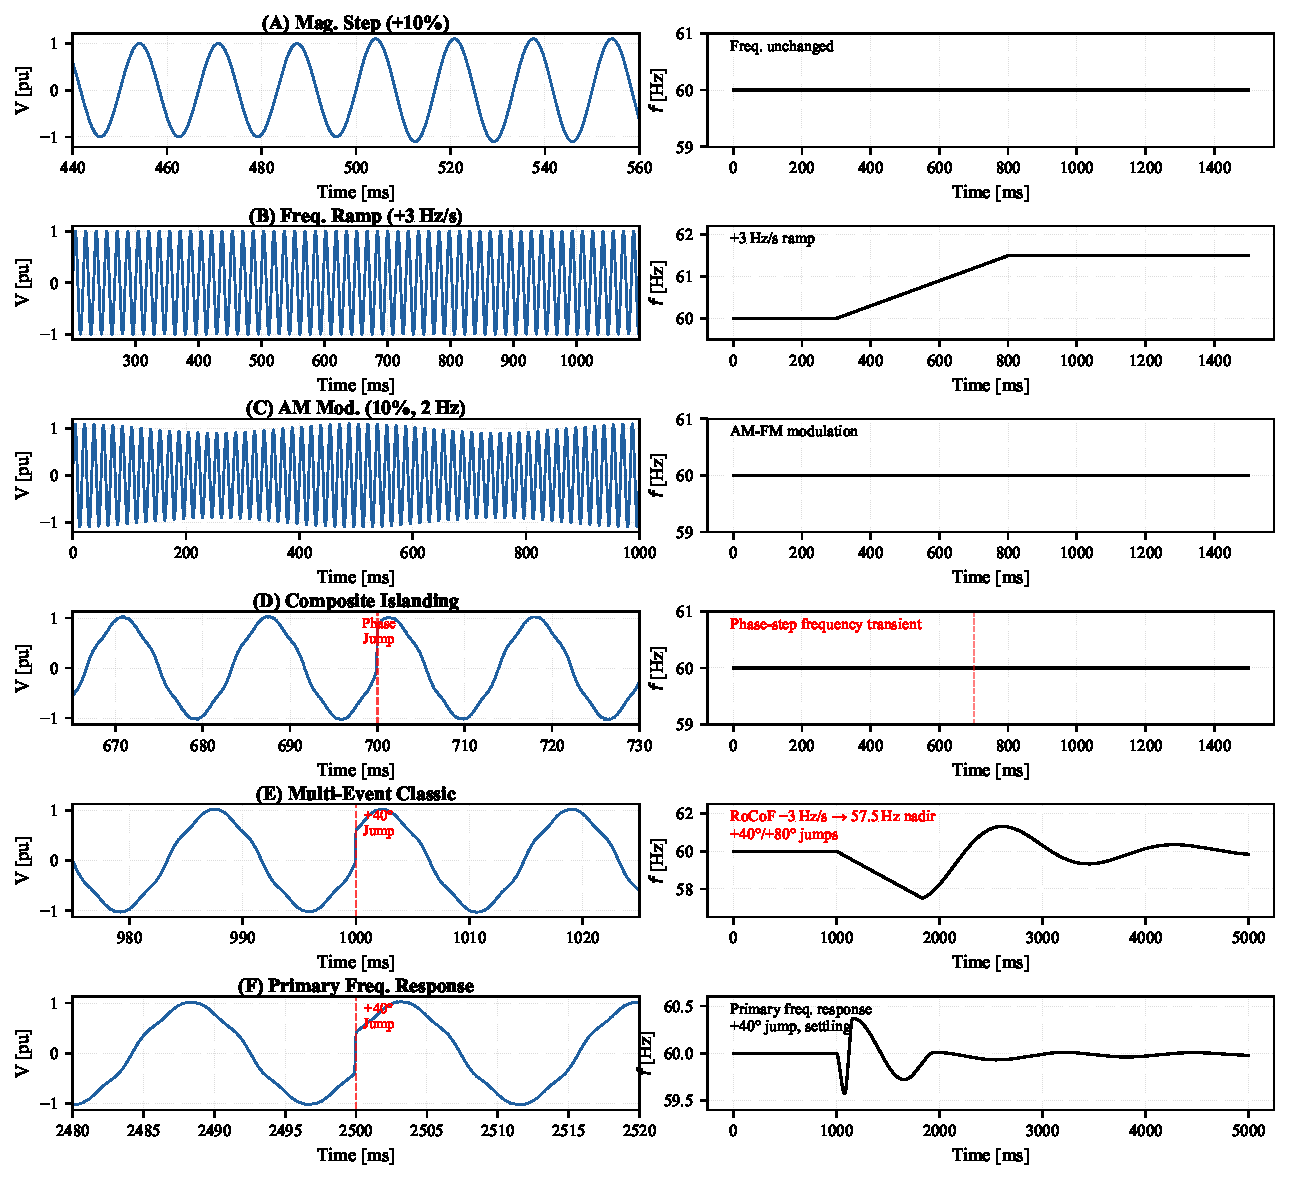
\includegraphics[width=0.99\textwidth]{Figures/Plots_And_Graphs/Fig1_Scenarios_Final.pdf}
    \caption{Complete Stress-Test Scenario Suite. (A–C) Dynamic performance
        profiles following the test philosophy of IEC/IEEE~60255-118-1
        (step, ramp, modulation). (D) Composite Islanding featuring an
        instantaneous $+60^\circ$ phase jump with harmonics and elevated noise
        ($\sigma = 0.005$\,pu; Section~\ref{sec:scenarios}).
        (E) IBR Multi-Event: scenario-dependent noise ($\sigma_\text{base}=0.003$\,pu
        plus sparse impulsive spikes $\leq 0.05$\,pu); frequency profile shows
        the full 5\,s composite sequence.}
    \label{fig:scenarios}
\end{figure*}